\clearpage

\section{MPGVAE}\label{sec:MPGVAE}\index{MPGVAE}

\begin{notebox}
\textbf{Paper: } \fullcite{flam-shepherd_mpgvae_2021}
\vspace{5pt}

no reviews
\hspace{1cm}
no official code
\hspace{1cm}
\href{Flam-Shepherd et al_2021_MPGVAE.pdf}{Local pdf}
\vspace{3pt}

Read for Yoann's\index{Yoann} work 5/2/2022
\hfill Notes taken: 6/2/2022 \index{February 2022}
\end{notebox}

\begin{notebox}[colback=red!5]
\tldr Builts on GraphVAE (Simonovsky and Komodakis, 2018) but bypasses the graph matching problem by relaying on message passing NN in encoder and decoder so that the reconstruction loss can be calculated directly. Message passing over edges, nodes use attention to aggregate these.
To get from node representation to laten vector they use set2vec\index{set2vec} from Vinyals 2015 to be invariant to the node ordering.
To get from latent back to graph they use simply linear layer and then message passing, finishing with softmax over node and egde representation to create stochastic edge and node graph representations from which the graphs can be samples (in practice assume by max category).
The reconstruction loss assumes independence of node and edge features $p\theta(G|z) = \Pi_{v \in G} p(x_v | z) \Pi_{u \in G} p(e_{uv} | z)$
\end{notebox}

\begin{notebox}[colback=yellow!5]
\textbf{Notes:} 
\begin{itemize}[nosep]
\item code not publicly available - asked first author, no answer
\item set2vec to be invariant to node ordering when getting from the node representation in the last MPNN layer the latent representation $z$, on the way back can use use MLP and MPNN cause the ordering problem was solved when moving to the latent
\item \emph{\textbf{I still do not see how the reconstruction loss can be evaluated. Even with the independence assumptions, each of the node/ edge likelihoods has to be matched to the respective edge/ node in the original graph. How can this be done without some matching procedure?}}
\end{itemize}
\end{notebox}


Graph with adjacency matrix, edge feature tensor and node feature matrix $G = (A, E, X)$.
Assume independence between node and edge probability distributions (Erdos-R\'enyi graph model) such as in \citetitle{simonovsky_graphvae_2018} of \textcite{simonovsky_graphvae_2018}\index{GraphVAE}.

Starting point is standard VAE and ELBO. Both edge and node features are categorical.
Build a message passing NN (MPNN)\index{message passing NN} into encoder and decoder of the VAE.

Refers to Graphite from Grover et al 2018 as nearest baseline - how different is this?

\begin{figure}[ht]
\centering
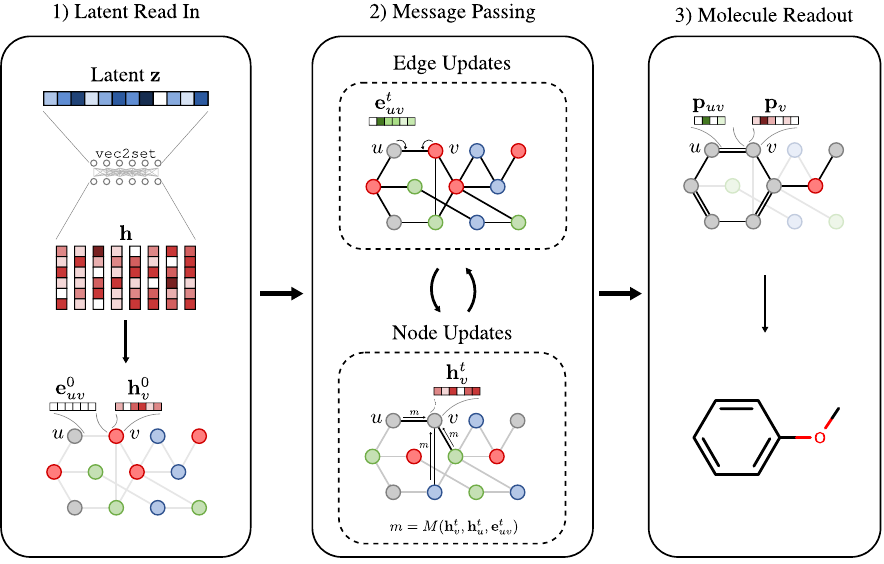
\includegraphics[width=10cm]{mpgvae_figure1.png}
\caption{1) Read in latent $z$ by passing it through linear layer to get to correct node dimensions and pass it through RNN to get initial node featues. Edge features fixed to zero - unconnected graph. 2) Message passing on both, node and edge representations. 3) Use last node and edge representation to predict independent node and edge feature probabilities.}
\end{figure}

Claim that has lower complexity than GrpahVAE (how so?).

\textbf{Encoder:} Use MPNN to map node and edge representations into latent space.
Messages are constructed at edge level as linear functions of itself, neighbouring nodes, and edge features passed through tanh nonlinearity.
Edge updates are directly the messages. 
Node updates first use attention to reweight the messages and then pass it through a GRUCell (this is not very clear, there is something strange in eq. 11 - should be a message for u only? not uv?)
Use set2set from Vinyals 2015 (unlike in seq2seq, in sets the order should not matter and the model should produce the same representation in arbitrary ordering of the set) to read from last node representation to fixed-sized hidden representation $z$.

\textbf{Decoder:} Pass latent through linear layer to expand dims and then RNN to get initial node featurs (edge features zero - unconnected graph). MPNN identical to encoder - update both nodes and eges.
Readout the last layer into stochastic graph representation by passing it through single layer NN and softmax.

\textbf{Experiments:} Over QM9 (not clear whether kekulized or not and if has hydrogens) - best validity compared to GrphVAE, MolGAN, CharacterVAE and Grammar VAE. Generate $10^4$ molecules and achieve validity over 90\%, unique almost 70\% and novel about 50\% - much better then baseline. 
Also evaluates the continuous (chemical properties) and discrete (avg number of atom types and ring size) property distributions of generated vs training sample graphs - claim to have both better than baseline.



